\newcommand{\modelreality}{Modelering af Virkeligheden}
\newcommand{\topicone}{Aalborg PBL}
\newcommand{\topictwo}{Representation}
\section*{\modelreality}

\begin{frame}{\modelreality}
\begin{itemize}
	\item \topicone
	\item \topictwo
\end{itemize}
\end{frame}

\subsection*{\topicone}

\begin{frame}{\topicone} 
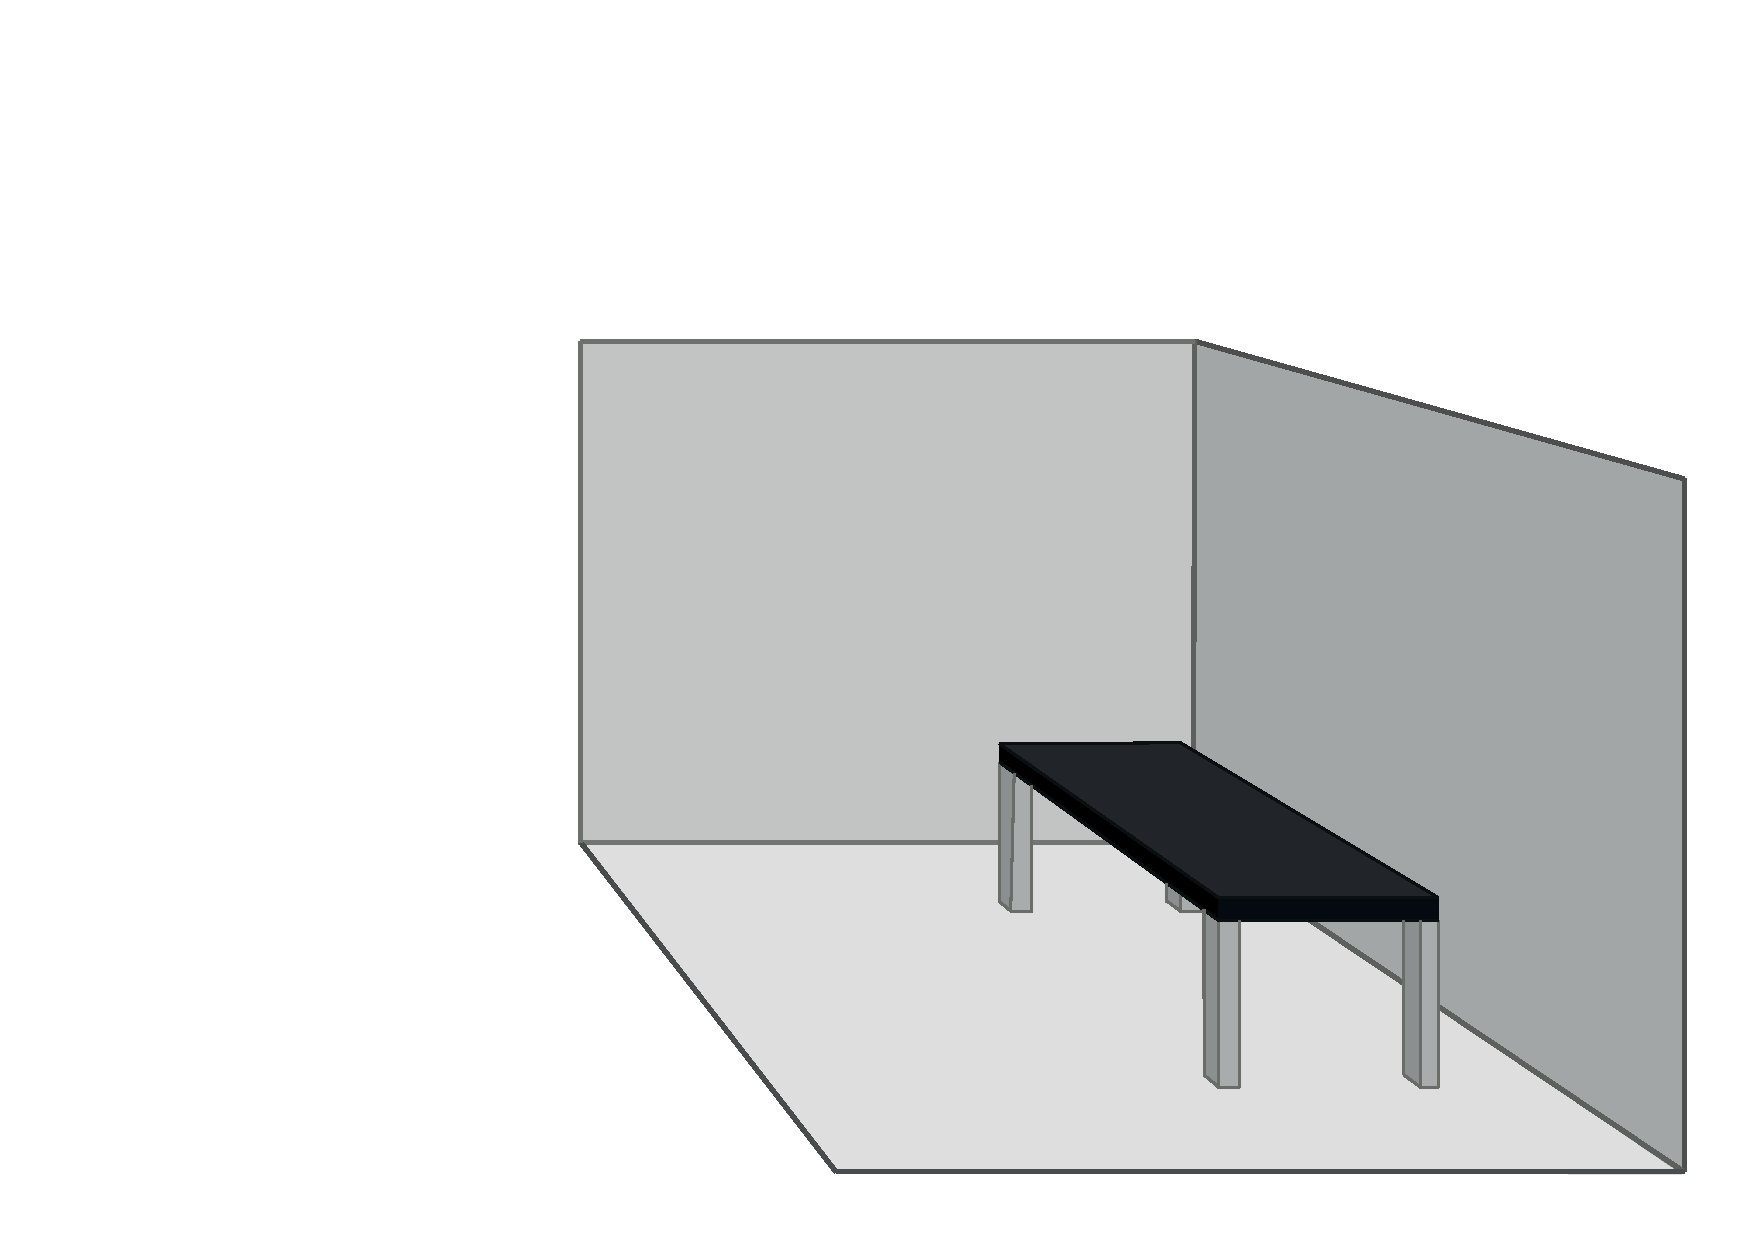
\includegraphics[width=\columnwidth]{input/rasmus/Rasmus1.pdf}
\end{frame}

\begin{frame}{\topicone} 
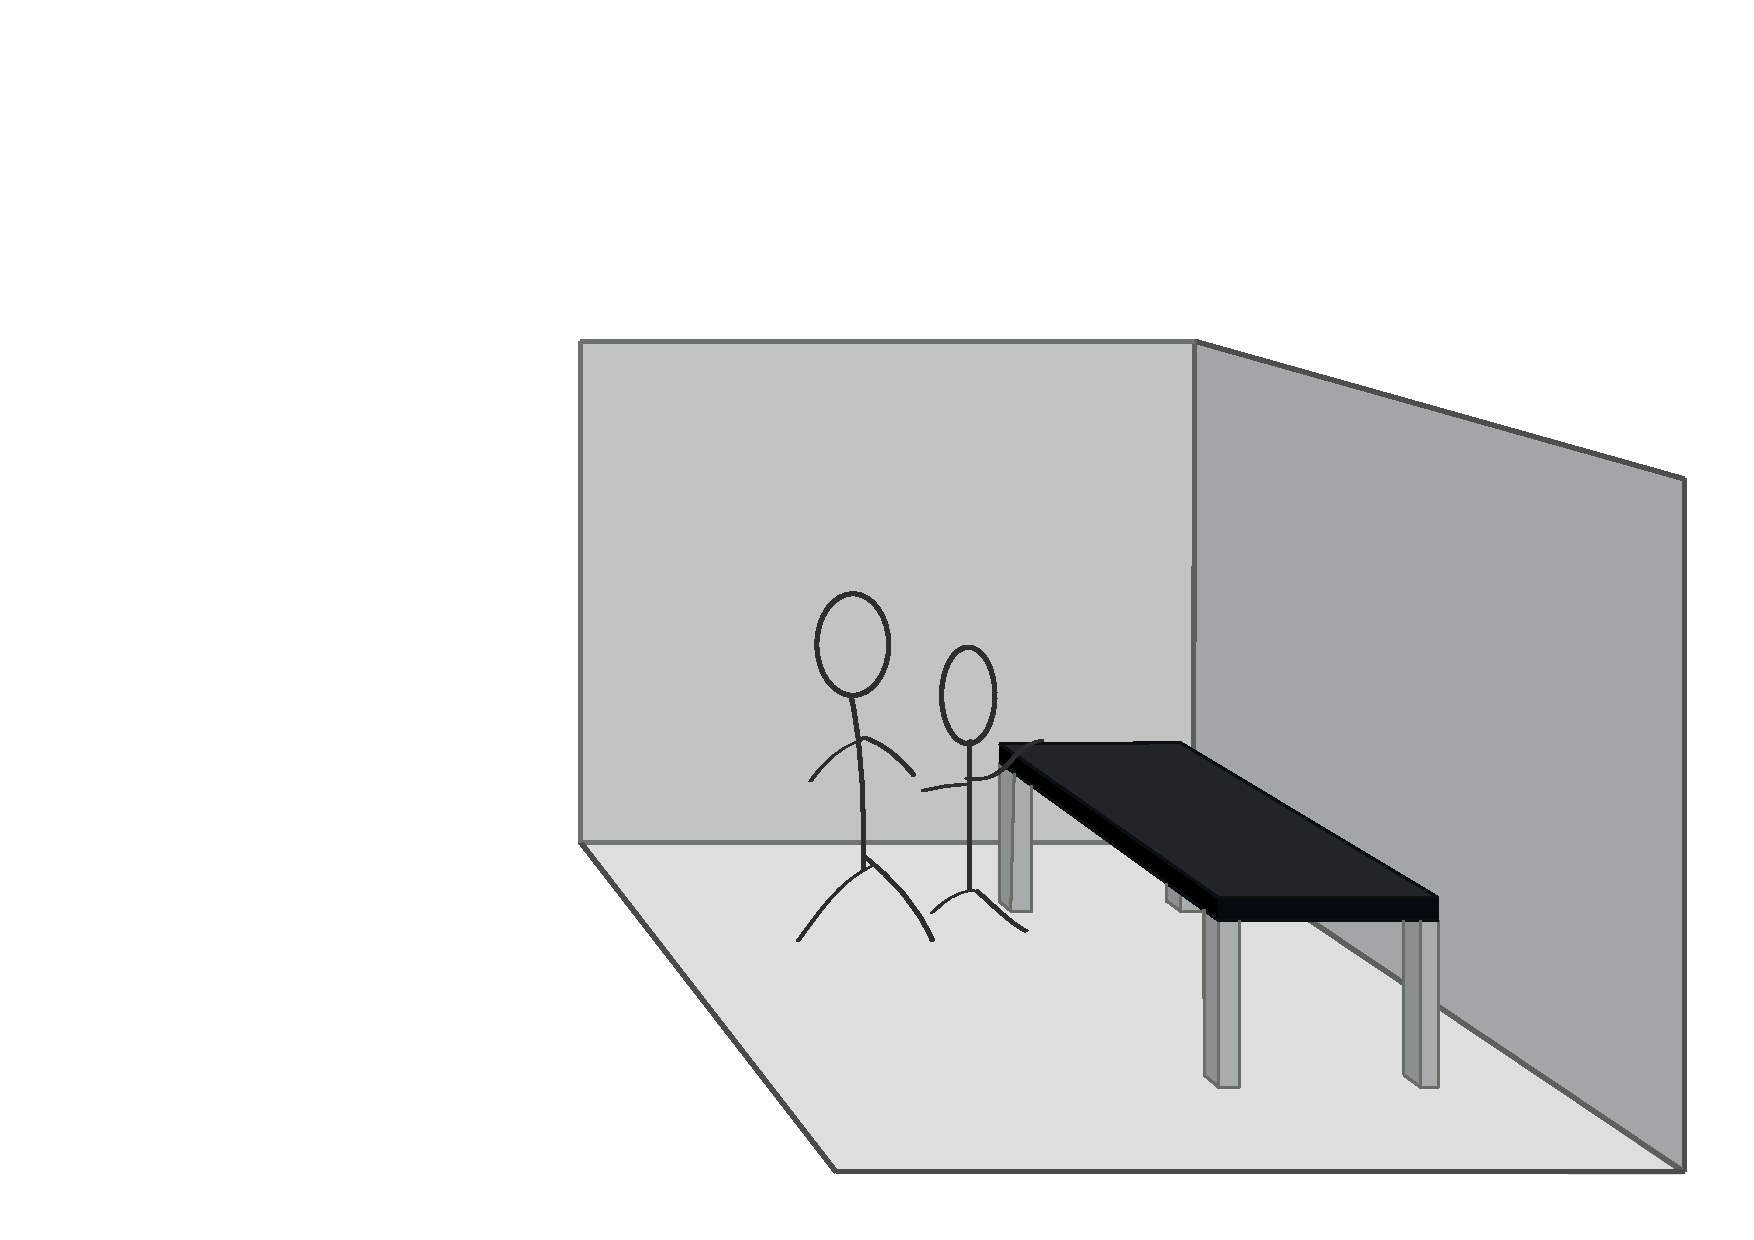
\includegraphics[width=\columnwidth]{input/rasmus/Rasmus2.pdf}
\end{frame}

\begin{frame}{\topicone} 
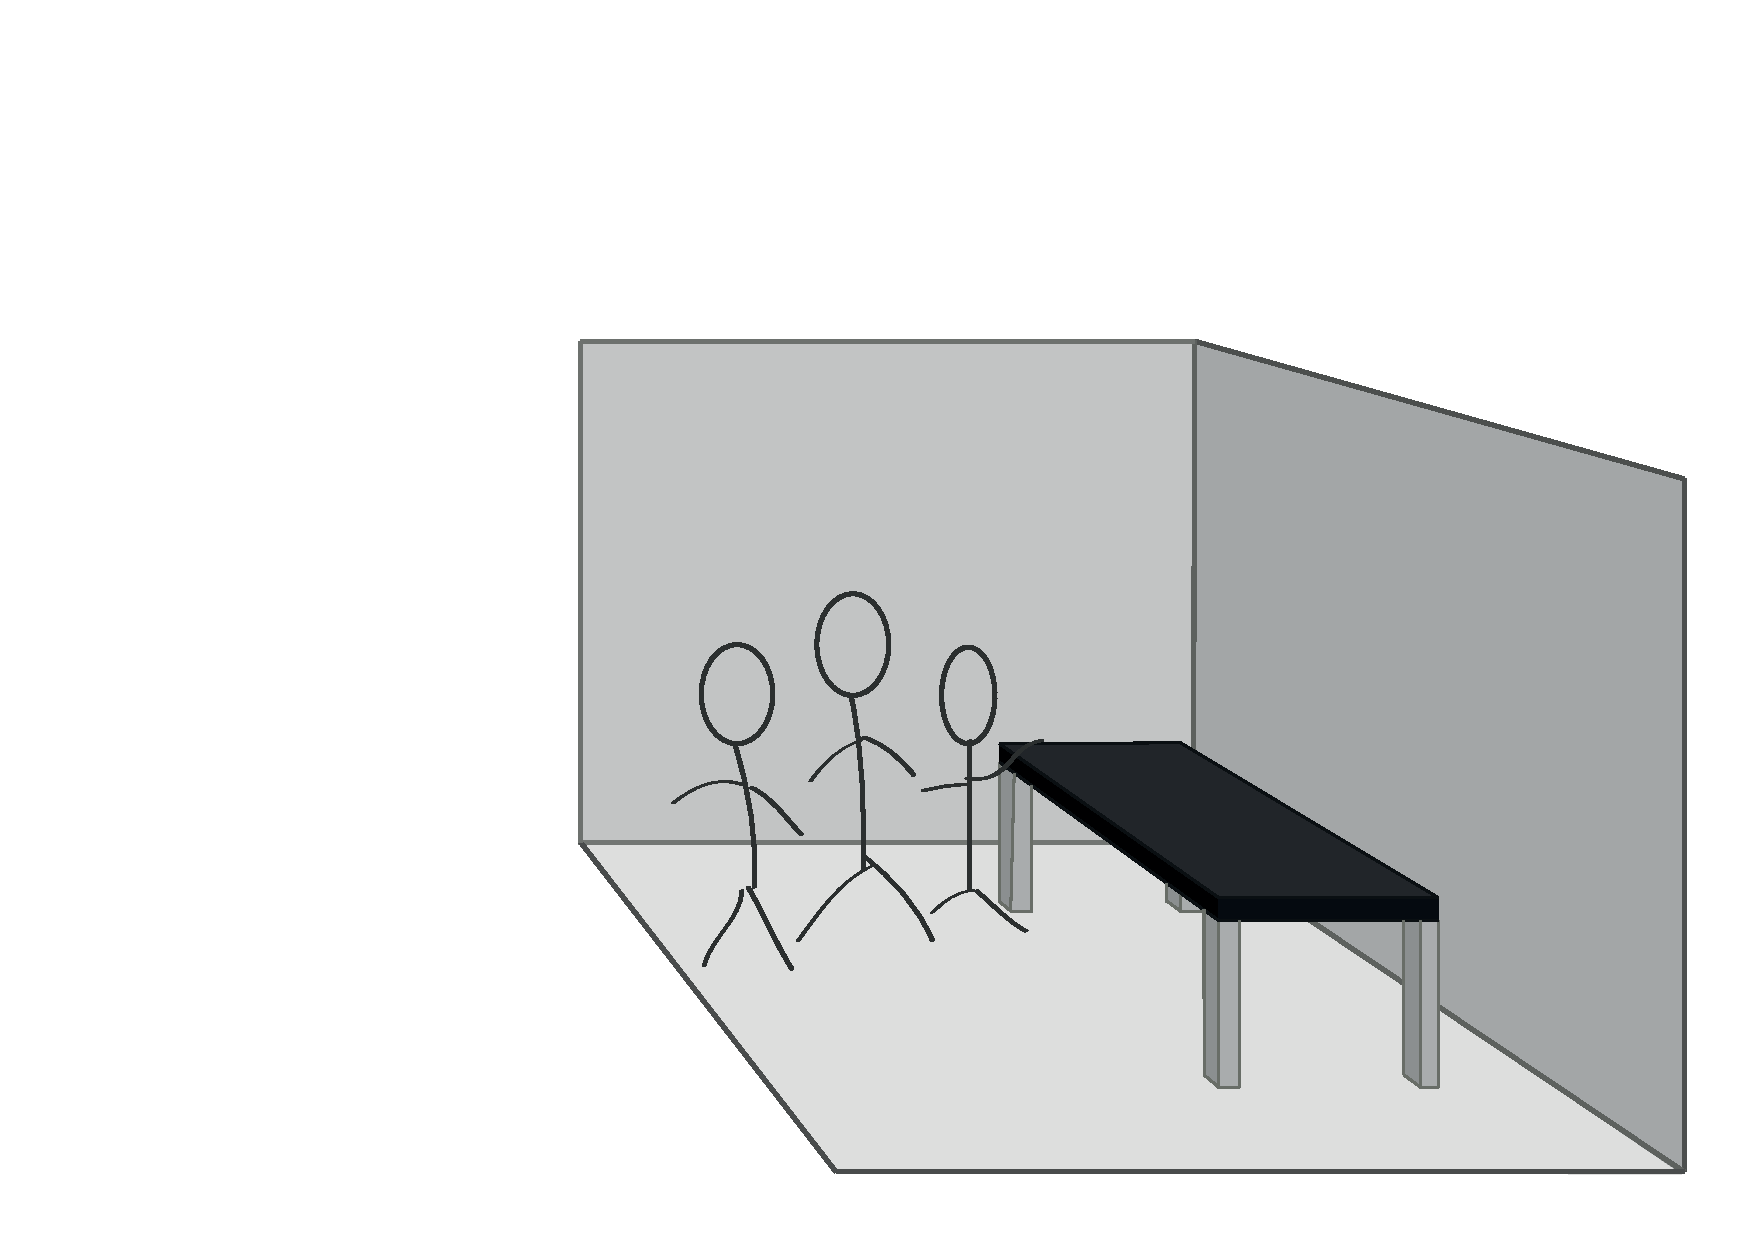
\includegraphics[width=\columnwidth]{input/rasmus/Rasmus3.pdf}
\end{frame}


\begin{frame}{\topicone} 
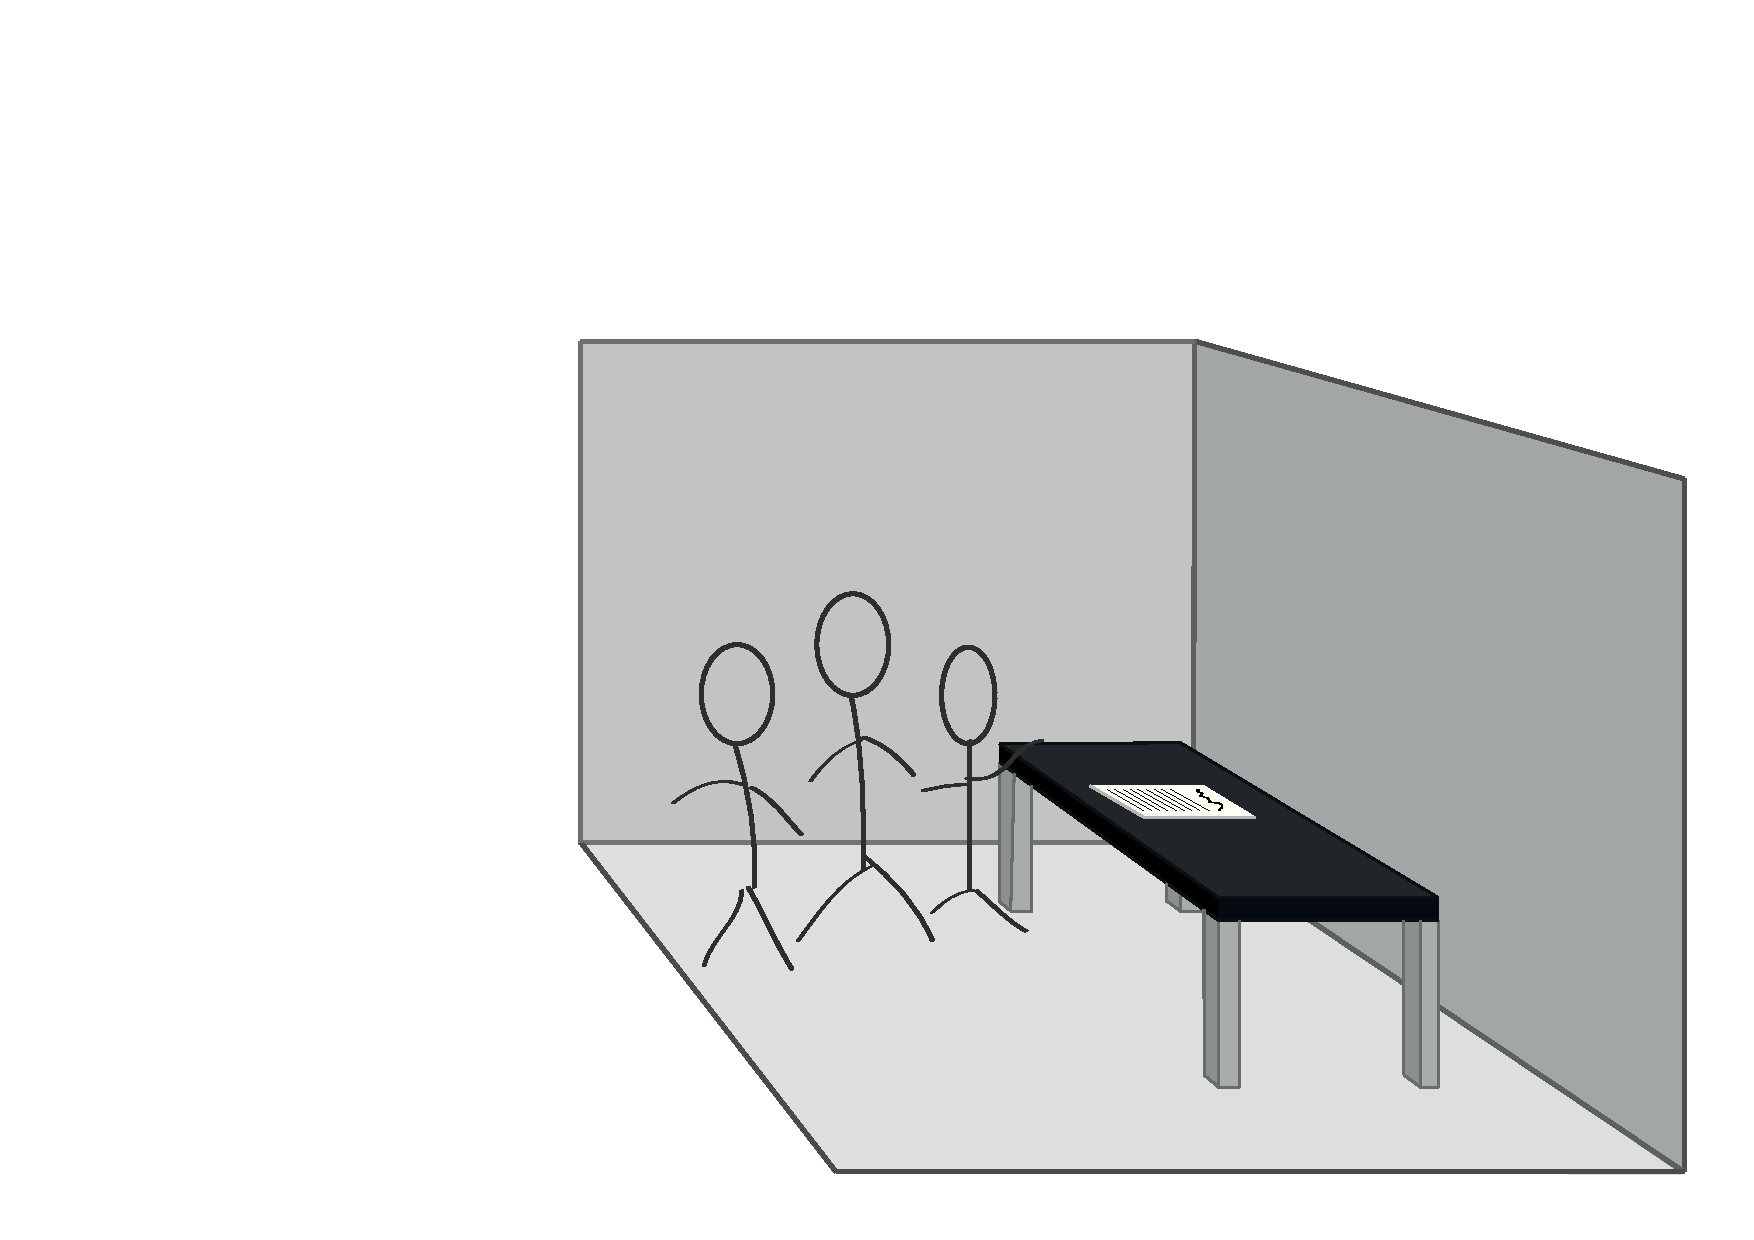
\includegraphics[width=\columnwidth]{input/rasmus/Rasmus4.pdf}
\end{frame}


\begin{frame}{\topicone} 
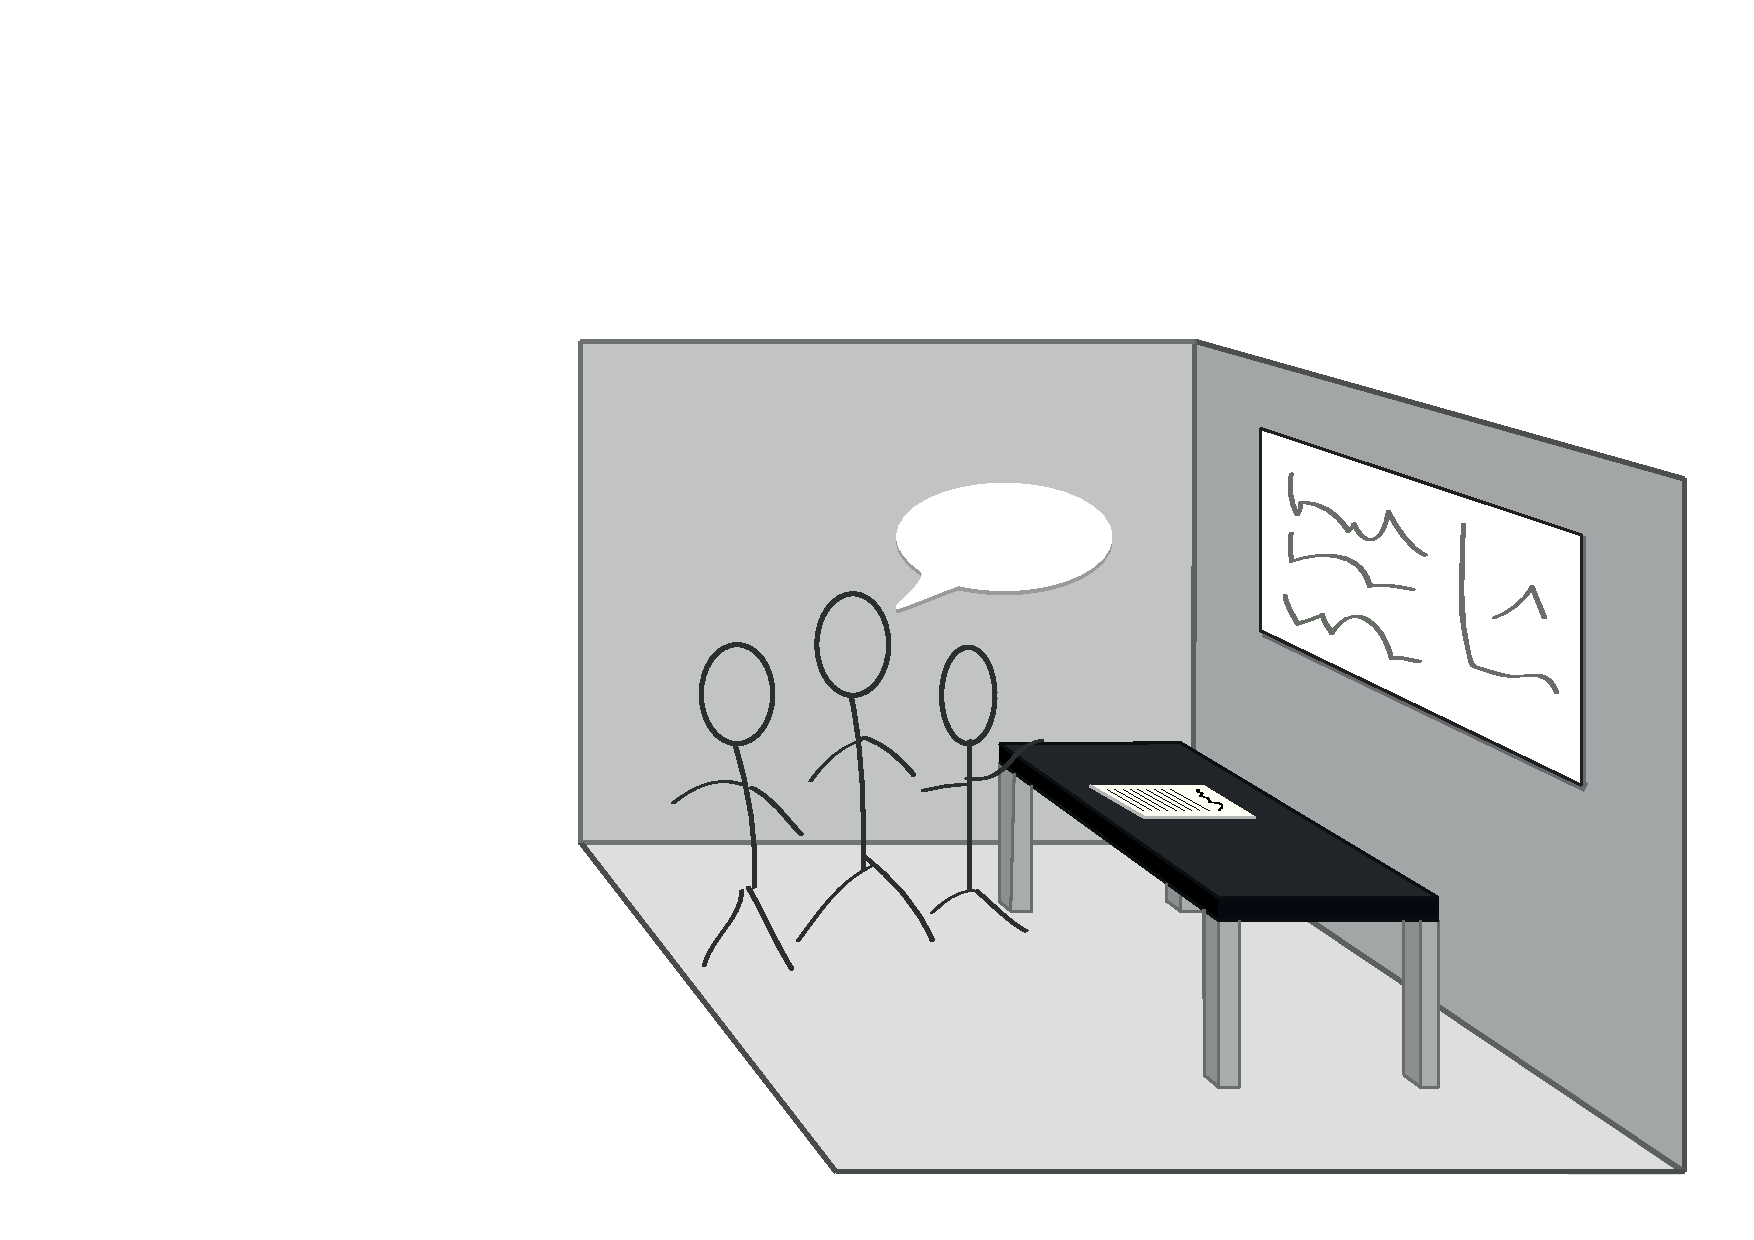
\includegraphics[width=\columnwidth]{input/rasmus/Rasmus5.pdf}
\end{frame}


\begin{frame}{\topicone} 
\includegraphics[width=\columnwidth]{input/rasmus/Rasmus6.pdf}
\end{frame}




\subsection*{Rutebestemmelse}

\begin{frame}{Rutebestemmelse} %s�tte hjulene i rette position

\end{frame}

\begin{frame}{Rutebestemmelse} 
\includegraphics[width=\columnwidth]{input/styring/4.png}
\end{frame}

\begin{frame}{Rutebestemmelse} %billede s 17
\includegraphics[width=\columnwidth]{input/styring/6.png}
\end{frame}